\subsection{Monte Carlo Backgrounds}
\label{sec:mcbg}

Details of the MC based background estimations are described below.
Any additional normalizations or uncertainties are summarized
in Table~\ref{tab:mcnorm}.

\begin{table}[htp]
\centering
    \begin{tabular}{|c|cc|}
    \hline
    Background & Normalization Factor & Unceratinty \\ 
    \hline\hline
    $WZ$ & 1.08 & 10~\% \\
    $ZZ$ & 1.05 & 15~\% \\
    %$Z\gamma$ & & 30~\% \\
    $\ttbar +V$ & 1.0 & 30~\% \\
    $ZWW+ZZZ$ & 1.0 & 50~\% \\
    \hline
  \end{tabular}
  

\caption{Summary of normalizations and their uncertainties for the
MC based background estimates used in the analysis.}
\label{tab:mcnorm}
\end{table}



\subsubsection{$WZ$}
\label{sec:wzbg}

\paragraph{Introduction}
The $WZ$ process constitute an irreducible background for the $WWW$ final state. Studies of this final state have been performed at the LHC by the ATLAS~\cite{Aad:2012twa,Anger:1663539} and CMS~\cite{CMS-PAS-SMP-12-006} collaborations. They have shown that the measured cross-section is systematically found to be higher than the NLO predictions, by a factor of about $\approx{}10-15\%$. The recent cross-sections calculations at NNLO for the $V\gamma$ processes~\cite{Grazzini:2015nwa} have shown that the expectations are corrected by a large factor compared to the one at NLO. Similar conclusions also apply for the $ZZ$ final state~\cite{Cascioli:2014yka}. However these predictions are not yet available for the $WZ$ process. Therefore the NLO predictions for this background, must be checked from the data. In the following a correction factor to MC predictions will be derived from the data using a 2D sideband method. To simplify the explanations, in this section, the $WZ$ process will be considered as the signal process.
% It is therefore very important to determine the normalization of this background using data.

The normalization of this process is determined from data using a two-dimensional sideband method (2D sideband method or so-called ABCD method~\cite{Aad:2013izg}). Events are requested to pass the event pre-selection and contain exactly one SFOS lepton pair, and one third lepton from a different flavor. In order to supress contributions from fake-lepton backgrounds as much as possible, all leptons must satisfy the following transverse momentum requirement: $p_{T}>25~\GeV$. The two dimensions of the method are defined as the invariant mass of the two SFOS leptons on one axis and the isolation of the non-SFOS lepton as the other one. This leads to 4 regions defined as follows:

\begin{itemize}
	\item Signal Region (A): Isolated and in Z-peak $|m_{\ell\ell}^{SFOS}-m_{Z}|<15~\GeV$, $E_{T}^{Iso(R<0.2)}/E_{T}<0.10$ and $p_{T}^{Iso(R<0.2)}/p_{T}<0.04$.
	\item Control Region (B): Isolated and off Z-peak $|m_{\ell\ell}^{SFOS}-m_{Z}|>25~\GeV$, $E_{T}^{Iso(R<0.2)}/E_{T}<0.10$ and $p_{T}^{Iso(R<0.2)}/p_{T}<0.04$.
	\item Control Region (C): Non-isolated and in Z-peak $|m_{\ell\ell}^{SFOS}-m_{Z}|<15~\GeV$, $E_{T}^{Iso(R<0.2)}/E_{T}>0.15$ and $p_{T}^{Iso(R<0.2)}/p_{T}>0.10$.
	\item Control Region (D): Non-isolated and off on Z-peak $|m_{\ell\ell}^{SFOS}-m_{Z}|>25~\GeV$, $E_{T}^{Iso(R<0.2)}/E_{T}>0.15$ and $p_{T}^{Iso(R<0.2)}/p_{T}>.10$.
	
\end{itemize}


The 2D-sideband method is based on the following two assumptions:
\begin{itemize}
\item The presence of $WZ$ signal events in the three control regions (B,
  C, and D) is negligible. This allow us to consider all
  reconstructed leptons falling in one of these regions as coming from a
  background (non $WZ$)event. The number of events $N^{jet}$ with jet faking leptons can then
  be extracted by subtracting from the data the contribution from processes containing 
  3 real leptons ($ZZ$, $ttV$, triboson) or 2 real lepton and 1 photon ($Z\gamma$)
  and noted in the following as $N^{EW}$. These are estimated from Monte Carlo. The total number of
  observed events in each of these three regions can be expressed as:
  \begin{align}
  N_A &= N_A^{WZ}(measured)+N_A^{jet}+N_A^{EW} \\
  N_B &= N_B^{jet}+N_B^{EW} \\
  N_C &= N_C^{jet}+N_C^{EW} \\
  N_D &= N_D^{jet}+N_D^{EW} 
  \end{align}

\item The ratio of isolated to non-isolated background candidates from
  jet-fakes in the Z-peak bin ($\frac{N_D^{jet}}{N_C^{jet}}$)
  is equal to the same ratio computed in the off Z-peak bin ($\frac{N_B^{jet}}{N_A^{jet}}$).
\end{itemize}

From these equations, the number of $WZ$ events in the signal region A can be calculated as:

\begin{equation}
N_A^{WZ}(Measured)=(N_A-N_A^{EW})-\frac{1}{R^{jet}} \frac{(N_B-N_B^{EW}-c_B (N_A^{WZ}(MC))) (N_C-N_C^{EW}-c_C (N_A^{WZ}(MC)))}{N_D-N_D^{EW}-c_D (N_A^{WZ}(MC))}
\label{Equ:NWjet1}
\end{equation}

Where 
\begin{itemize}
\item $R^{jet}=\frac{N^{jet}_B N^{jet}_C}{N^{jet}_A
  N^{jet}_D}$ is defined to account for the bias on the background correlation between region A-B to C-D. These numbers are estimated from MC simulations, they are obtained from summing together samples containing 2 real leptons and a fake lepton ($Z+$jets, $t\bar{t}$ and $WW$). The MC samples used for these processes are summarized in Tables~\ref{tab:sample_bkg_dibosons},~\ref{tab:sample_bkg_dibosons_gg2DPI}, and~\ref{tab:sample_bkg_Zjets} in Section~\ref{sec:subsection_datasets_MC}.
\item $C_X=\frac{N_X^{WZ}(MC)}{N_A^{WZ}(MC)}$, X=(B,C,D) is defined to account for the signal leakage. These numbers are estimated from MC simulations.
\item $N_X^{EW}$, X=(A,B,C,D), is evaluated from MC and defined as the number of events containing 3 real leptons ($ZZ$, $t\bar{t}V$, triboson) or 2 real lepton and 1 photon ($Z\gamma$).
\end{itemize}
The signal leakage $C_X$ is estimated using the signal $WZ$ Monte Carlo, whereas, when computing the measurement central value, the $R^{jet}$ factor is fixed to 1. A systematic uncertainty is associated to this assumption. 

\paragraph{Nominal estimate}


Table~\ref{tab:WZ_Nominal_Numbers} summarizes the number of events measured in all 4 regions.

\begin{table}[htp]
\centering
\begin{tabular}{c|cccc}
  \hline
  Regions & N data events & N EWbkg      & N fakes (MC)    & CX \\
  \hline
	    A & $724 \pm 27$ & $172 \pm 3$   & $25 \pm 4$ & $1 \pm 0$ \\ 
	    B & $67 \pm 8$   & $29 \pm  2$   & $5 \pm 2$ & $0.0639 \pm 0.0007$ \\ 
	    C & $272 \pm 16$ & $7.7 \pm 0.9$ & $282 \pm 12$ & $0.0018 \pm 0.0001$ \\ 
	    D & $118 \pm 11$ & $1.9 \pm 0.6$ & $103 \pm 7$ & $0.00019 \pm 0.00003$ \\ 
  \hline
\end{tabular}
\caption{Number of data and MC events reccorded in each regions, used for the determination of the $WZ$ normalization using the 2D-sideband method.}
\label{tab:WZ_Nominal_Numbers}
\end{table}

In region A the total predicted number of $WZ$ events is $N_A^{WZ}(MC)=498{}\pm 1$, while the measurement with the 2D-sideband method gives $N_A^{WZ}(measured)=537.\pm{}35$ events, this yield a correction factor of $1.08 \pm 0.07$(stat). This normalization factor is found to agree well with the measurements done by the ATLAS and CMS collaborations. 
The number of fake leptons events can also be evaluated with this method, subtracting the number of EW and $WZ$ events to the total number of data events in region A. Doing so, one find $N^{jet}_{A}(measured)=8. \pm 23.$, to be compared to the MC expectation of $N^{jet}_{A}(MC)=25 \pm 4.$. The error on this number is large, but since the contamination of fake events in this region A is small, the impact on the correction factor is also small.
% Due to the high contamination of $WZ$ and EW events in region B, the evaluation of the fake component has a large uncertainty. But this high uncertainty is counterblanced by the small fraction of events expected in th
% The way the 2d-sideband method is used The number of fake events measured in the data in region A is  $N^{jet}_{A}(measured)=8. \pm 23.$ to be compared with the expectation in MC: $N^{jet}_{A}(MC)=25 \pm 4.$.

Figure~\ref{fig:WZ_CR} shows the $m_{\ell\ell}^{SFOS}$ distribution for the two isolation regions. As it can be seen the backgrounds do not model perfectly the data, especially in the non-isolated region. It is important to notice that the fake backgrounds are here completely determined from Monte Carlo simulations, as well as the $WZ$ normalization.

\begin{figure}[htp]
\centering
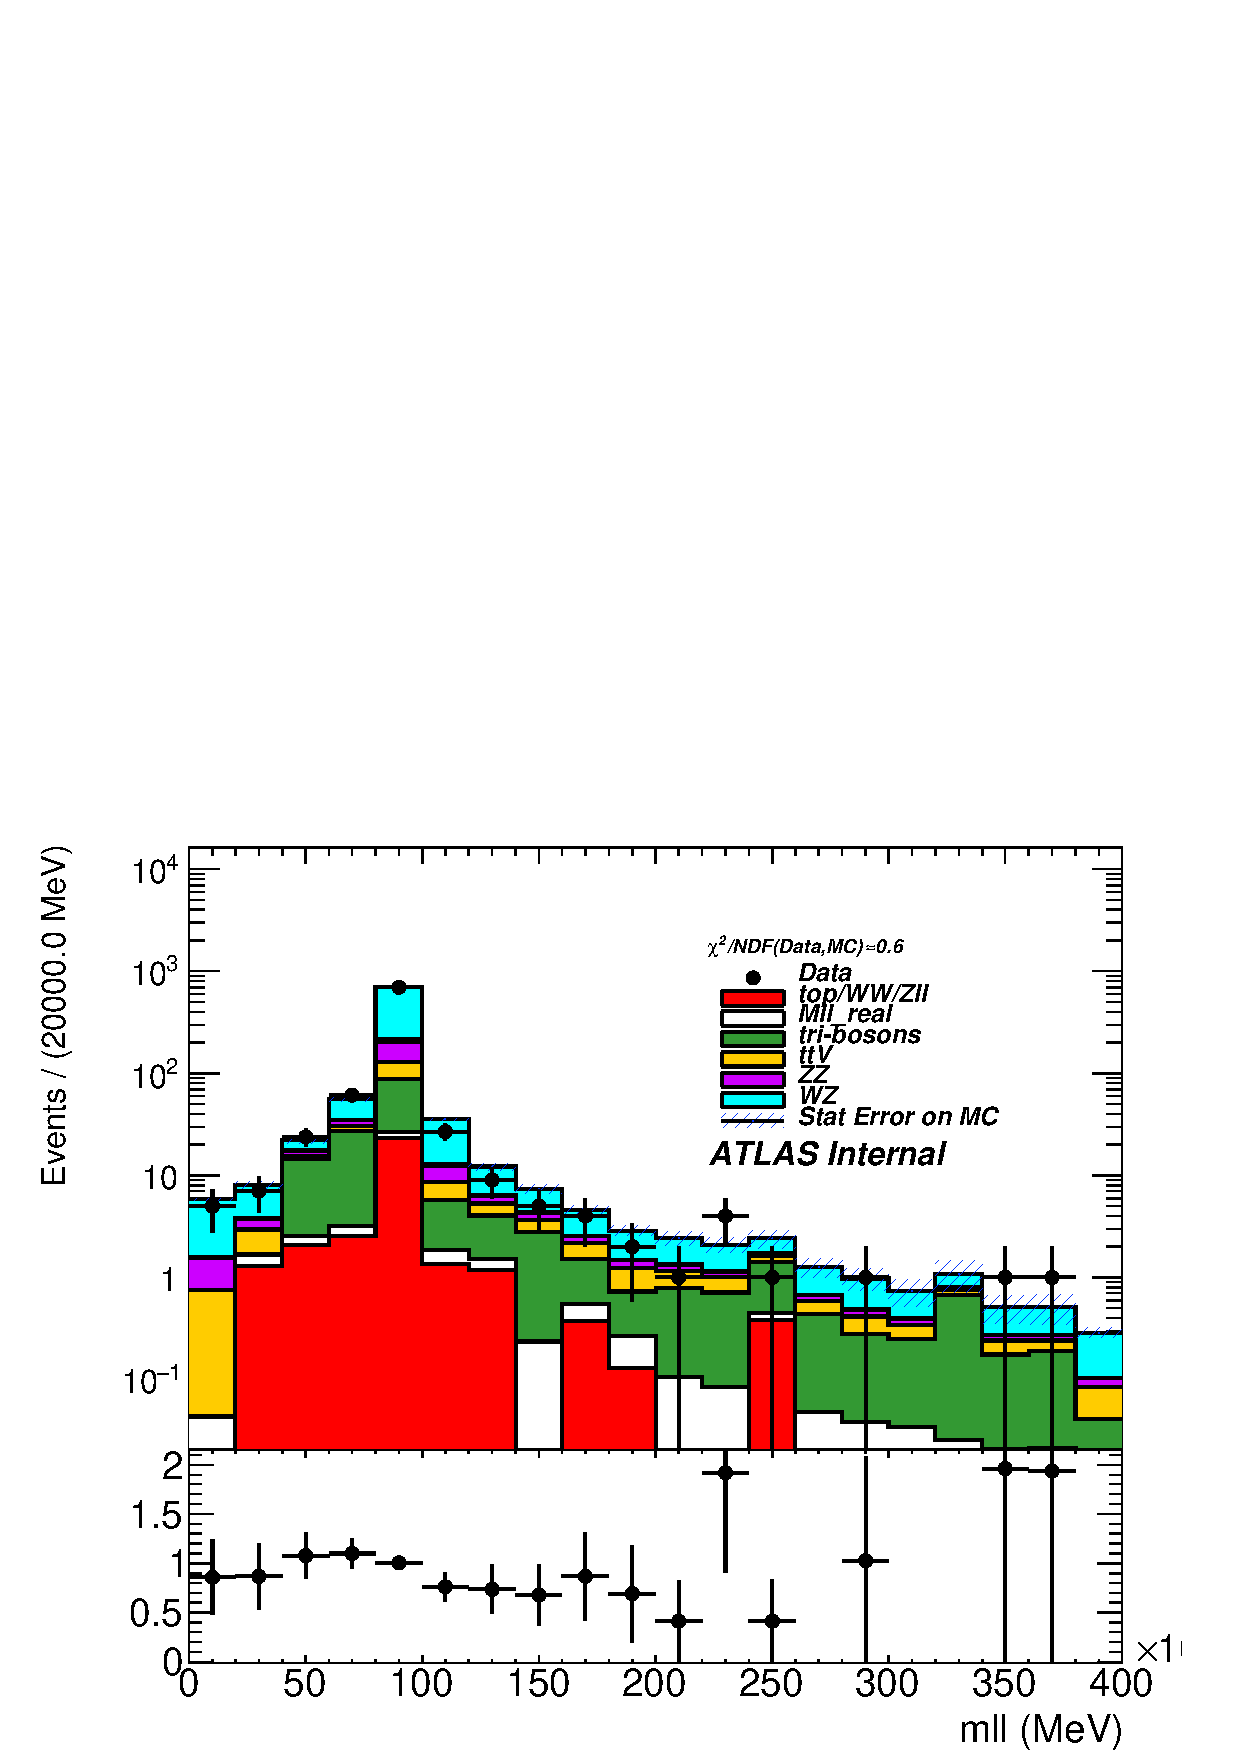
\includegraphics[width=0.45\textwidth]{figures/WZ_CR/2DSideband_WZCR_Isolated}
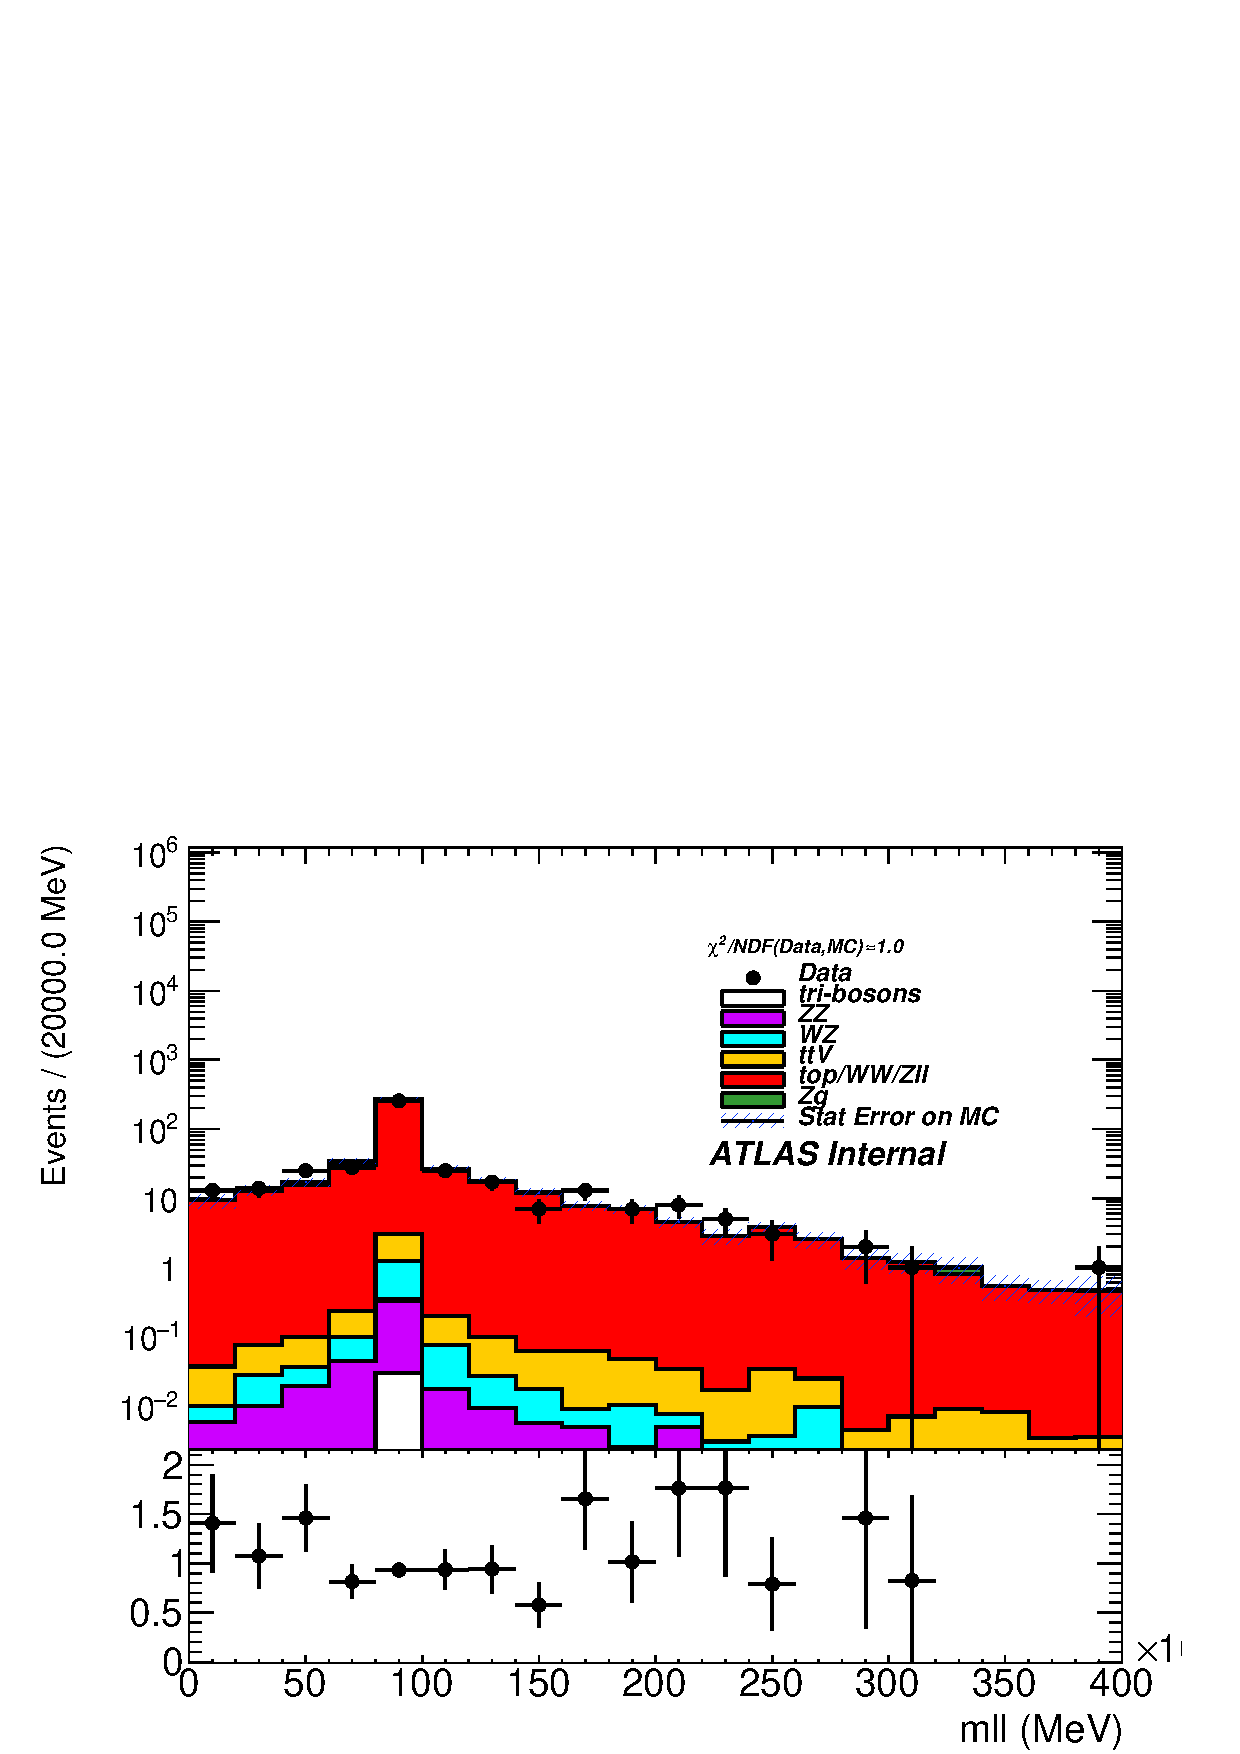
\includegraphics[width=0.45\textwidth]{figures/WZ_CR/2DSideband_WZCR_NonIsolated}
\caption{$WZ$ Control regions. Distribution of the $m_{\ell\ell}^{SFOS}$ in the isolated and anti-isolated CR.}
\label{fig:WZ_CR}
\end{figure}  

\paragraph{Closure test and systematic uncertainties}


To prove that the 2D-sideband method can determine accurately the $WZ$ normalization, MC closure tests are performed. The MC processes of the two isolations regions showed on Figure~\ref{fig:WZ_CR} are summed up. Two templates are obtained, and they are used as if they were data in region A, B, C and D. These templates are used to generate pseudo-datasets which will serve to recompute the number of $WZ$ events with the 2D-sideband method.
Once again the NLO prediction in region A gives $N_A^{WZ}(MC)= 498 \pm 1$, using the pseudo-data one find $N_A^{WZ}(measured)=495.\pm{}39$ events. Other tests are performed: 

\begin{itemize}
\item Scaling up the $WZ$ signal by $20\%$.
\item Scaling up the fake background by $50\%$.
\item Scaling up the EW background by $20\%$.
\end{itemize}

In all these cases the 2D-sideband method allows to retrieve the proper normalization of the $WZ$ signal injected. More information can be found in the Appendix~\ref{appendix:2dsideband}.



Several sources of systematic effects are investigated. The difference between the number of $WZ$ events measured in region A after varying one variable and the central value reported above is taken into account as a systematic. They are listed below, more details can be found in appendix~\ref{appendix:2dsideband}.
\begin{itemize}
\item The isolation cuts are varied to $E_{T}^{Iso(R<0.2)}/E_{T}>0.25$ and $p_{T}^{Iso(R<0.2)}/p_{T}>0.2$, in order to check the impact of this cut on the measured number of events. The total number of $WZ$ events found in this case is: $N_A^{WZ}(measured)=539 \pm 35$, which yield a systematic uncertainty of $0.5\%$ on the normalization factor.

% \item The $p_{T}$ cut on the 3rd lepton is varied by $\pm{}1~\GeV$, the largest deviation found is taken as a systematic on the normalization factor. It is found that the largest difference in the normalization factor is found when varying the lepton $p_{T}$ to $26~\GeV$. In this case the predicted number of events is found to be: $N_A^{WZ}(\mbox{MC})=468{}\pm 1$ while the measured number of events in the data is found to be $N_{\mbox{WZ}}^{\mbox{data}(Ori)} =492 \pm 34$, which yield a ratio of $1.05 \pm 0.07$, or a difference of $2.9\%$ with the nominal normalization factor.
 
\item The cut on the $m_{\ell\ell}$ is increased to $35~\GeV$ in the definition of region B and D. The total number of $WZ$ events found in this case is: $N_A^{WZ}(measured)=557. \pm 35$ , which yield a ratio of $1.12 \pm 0.07$, or a difference of $3.7\%$ with the nominal normalization factor.

\item The normalization of the backgrounds taken from MC, which are subtracted, is varied by $20\%$ up and down and the largest difference is taken as another systematic uncertainty. It is found that the largest uncertainty is obtained by varying up the normalization of these backgrounds. In this case one find $N_A^{WZ}(measured)=558 \pm 35$, which gives a ratio of $1.12 \pm 0.07$, or an uncertainty of $3.8\%$ compared to the central prediction.

 
\item Finally the $R^{jet}$ factor is varied from $R^{jet} =1.$ to the value measured in MC: $R^{jet} =0.61 \pm 0.24$. The uncertainty on this factor is quite large due to the very low statistics available in MC in the isolated control regions. $N_A^{WZ}(measured)=527. \pm 136.$, which gives a correction factor of $1.06 \pm 0.23$. This yield a systematic uncertainty of $2.4\%$ on the normalization factor.

\end{itemize}

All these uncertainties are added in quadrature giving a total systematic uncertainty of $5.9\%$ on the scale factor. The final correction factor on the normalization of the $WZ$ background is therefore: $k_{WZ}=1.08 \pm 0.07^{stat} \pm 0.07^{sys}$.

\paragraph{Validation}

In order to check the consistency of the scale factor determined above, the agreement between the data and the model is checked in a region passing the event pre-Selection cuts and containing exactly two SFOS lepton pairs. Figure~\ref{fig:WZ_2SFOS_CR} show the leading lepton \pt{}, the \MET{}, the invariant mass distribution of the two leading lepton \pt{}, and the jet multiplicity in this region. Table~\ref{tab:presel_2sfos_wzval} show the overall yields predicted by the model and observed on the data. The data agrees very well with the model in this region after using the k-factor presented above.

\begin{table}[ht!]
\centering
\begin{tabular}{|c||c|c|c|c|}
\hline
 & $eee$ & $ee\mu$ & $e\mu\mu$ & $\mu\mu\mu$\\ 
\hline\hline
$WZ$ &  $240.28 \pm 0.67$(stat) $\pm 21$(syst) &  $0.0 \pm 0$ &  $0.0 \pm 0$ &  $567.0 \pm 1$ $\pm 50$(syst)\\ 
$ZZ$ &  $60.07 \pm 0.13$ &  $0.0 \pm 0$ &  $0.0 \pm 0$ &  $91.48 \pm 0.17$\\ 
$Z\gamma$ &  $69.9 \pm 2.7$ &  $0.0 \pm 0$ &  $0.0 \pm 0$ &  $0.17 \pm 0.12$\\ 
$ZWW+ZZZ$ &  $0.435 \pm 0.019$ &  $0.0 \pm 0$ &  $0.0 \pm 0$ &  $0.864 \pm 0.028$\\ 
$t\bar{t}+V$ &  $4.845 \pm 0.044$ &  $0.0 \pm 0$ &  $0.0 \pm 0$ &  $10.509 \pm 0.066$\\ 
Fake (data-driven) &  $44.9 \pm 2.2$ &  $0.0 \pm 0$ &  $0.0 \pm 0$ &  $42.4 \pm 1.2$\\ 
$WWW$ &  $0.768 \pm 0.011$ &  $0.0 \pm 0$ &  $0.0 \pm 0$ &  $1.843 \pm 0.018$\\ 
\hline
Expected Background &  $420.4 \pm 3.5$ $\pm 21$(syst)&  $0.0 \pm 0$ &  $0.0 \pm 0$ &  $712.5 \pm 1.6$ $\pm 50$(syst)\\ 
Expected Signal + Background &  $421.2 \pm 3.5$ $\pm 21$(syst)&  $0.0 \pm 0$ &  $0.0 \pm 0$ &  $714.3 \pm 1.6$ $\pm 50$(syst)\\ 
\hline
Observed Data &  $425 \pm 21$ &  $0.0 \pm 0$ &  $0.0 \pm 0$ &  $757 \pm 28$\\ 
\hline
\end{tabular}

\caption{Expected and observed event yields binned by lepton flavor combination for the following selection: event pre-selection + 2 SFOS. Only the systematic uncertainties on the $WZ$ background due to the k-factor is given. The other uncertainties are only statistical.}
\label{tab:presel_2sfos_wzval}
\end{table}


\begin{figure}[htp]
\centering
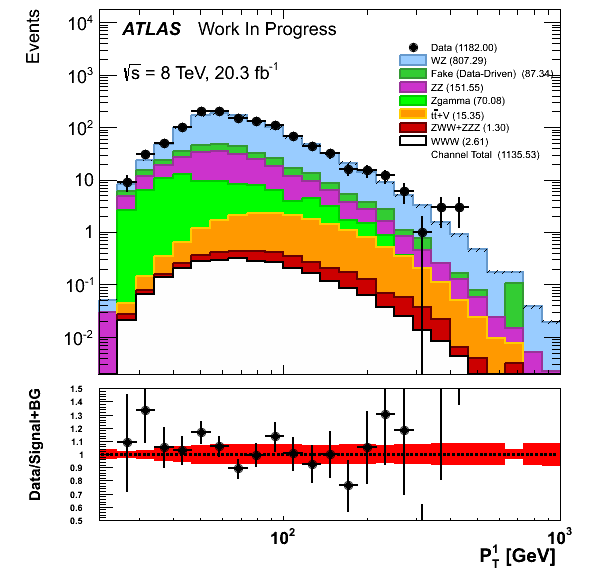
\includegraphics[width=0.4\textwidth]{figures/WZ_CR/LeadingLeptonPt_histratio.png}
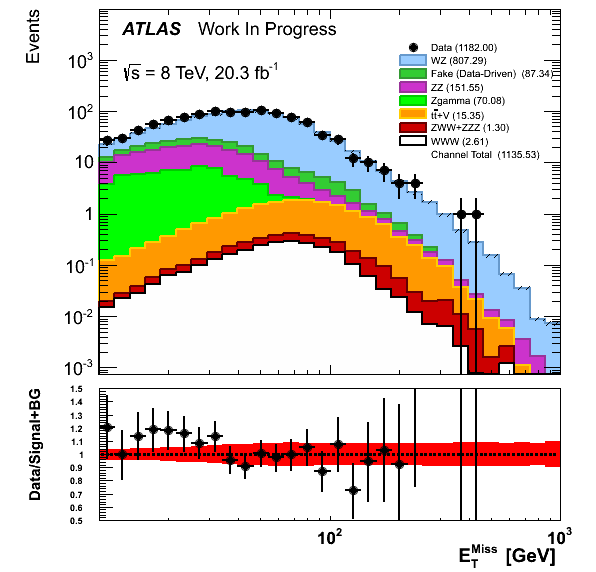
\includegraphics[width=0.4\textwidth]{figures/WZ_CR/MET_Et_histratio.png}
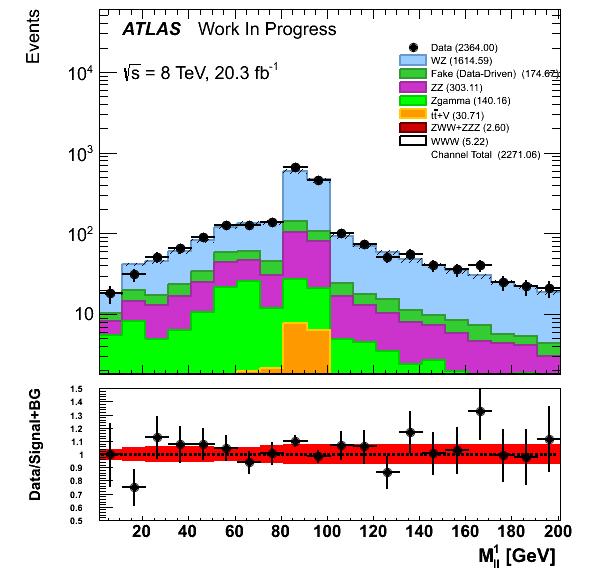
\includegraphics[width=0.4\textwidth]{figures/WZ_CR/InvariantMassSFOS_histratio.png}
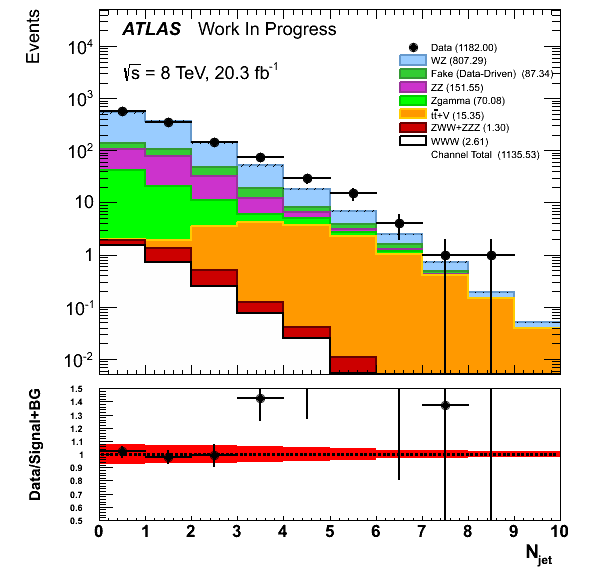
\includegraphics[width=0.4\textwidth]{figures/WZ_CR/NJets_histratio.png}

\caption{$WZ$ 2SFOS Control regions. Distribution of leading lepton $p_{T}$, $\MET$, $m_{12}$, and jet multiplicity. The systematic band shows the uncertainty on the WZ k-factor.}
\label{fig:WZ_2SFOS_CR}
\end{figure}  


\clearpage

\subsubsection{$ZZ$}
\label{sec:zzbg}

Another important process that participate to the 3 lepton final state, is due to the $ZZ^{*}$ production, where one lepton goes out of the detector acceptance, or doen't pass the selection criteria. The $ZZ^{*}$ backgrounds are modelled using the Powheg generator, and the $gg2ZZ$ generator for the loop induced processes. The normalization of the non-loop induced processes are scaled up to NNLO predictions using a kfactor which is 1.05, as defined in~\cite{Cascioli:2014yka,Baglio:2013toa,Bierweiler:2013dja}. The total systematic uncertainty associated to the theoretical predictions in this final state is taken to be $15\%$~\cite{Cascioli:2014yka,Baglio:2013toa,Bierweiler:2013dja}.

The agreement between data and the model is then checked in a control region, where 2 same flavors opposite sign pairs leptons ($e$ and $\mu$) are requested. The leptons must follow the quality requirements defined in Section~\ref{sec:Object_selection}. The transverse momentum of the leptons should be: $p_{T}^{1}>25~\GeV$, $p_{T}^{2}>15~\GeV$, $p_{T}^{3}>15~\GeV$, and  $p_{T}^{4}>10~\GeV$. The pairing of the leptons follows the algorithm defined in~\cite{Aad:2014wra}. In order to remove any contribution from fake backgrounds, only the events where the two $Z$ bosons are on shell are kept, \textit{ie}: $60<m_{12}<120~\GeV$ and $60<m_{34}<120~\GeV$. Figure~\ref{fig:ZZ_CR}, show the distributions of $m_{12}$, $m_{34}$, $m_{4l}$, and the leptons $p_{T}$ for this selection, while Table~\ref{tab:ZZ_CR} gives the total number of event measured in this CR and the prediction on the different processes in the same region.

The agreement between the data and the MC predictions is very good, for the shape or for the prediction of the total number of events in this control region.

It was also checked whether or not the contribution of $ZZ^{*}$ where the $Z^{*}$ boson is very offshell, $m_{Z^{*}} < 4$~GeV, while the other boson
has a  mass $m_Z > 4$~GeV has any impact on the signal regions. This was evaluted by looking at the samples with channel numbers
$181471$ through $181479$ in Table~\ref{tab:sample_bkg_dibosons}.  The contribution from these samples were found to be negligible, with a statistical
uncertainty compatible with exaxtly 0 events in the individual signal regions. As a result, these samples were not considered any further and are not
included in the final background  estimate for the signal regions or in the ZZ control regions.


\begin{figure}[htp]
\centering
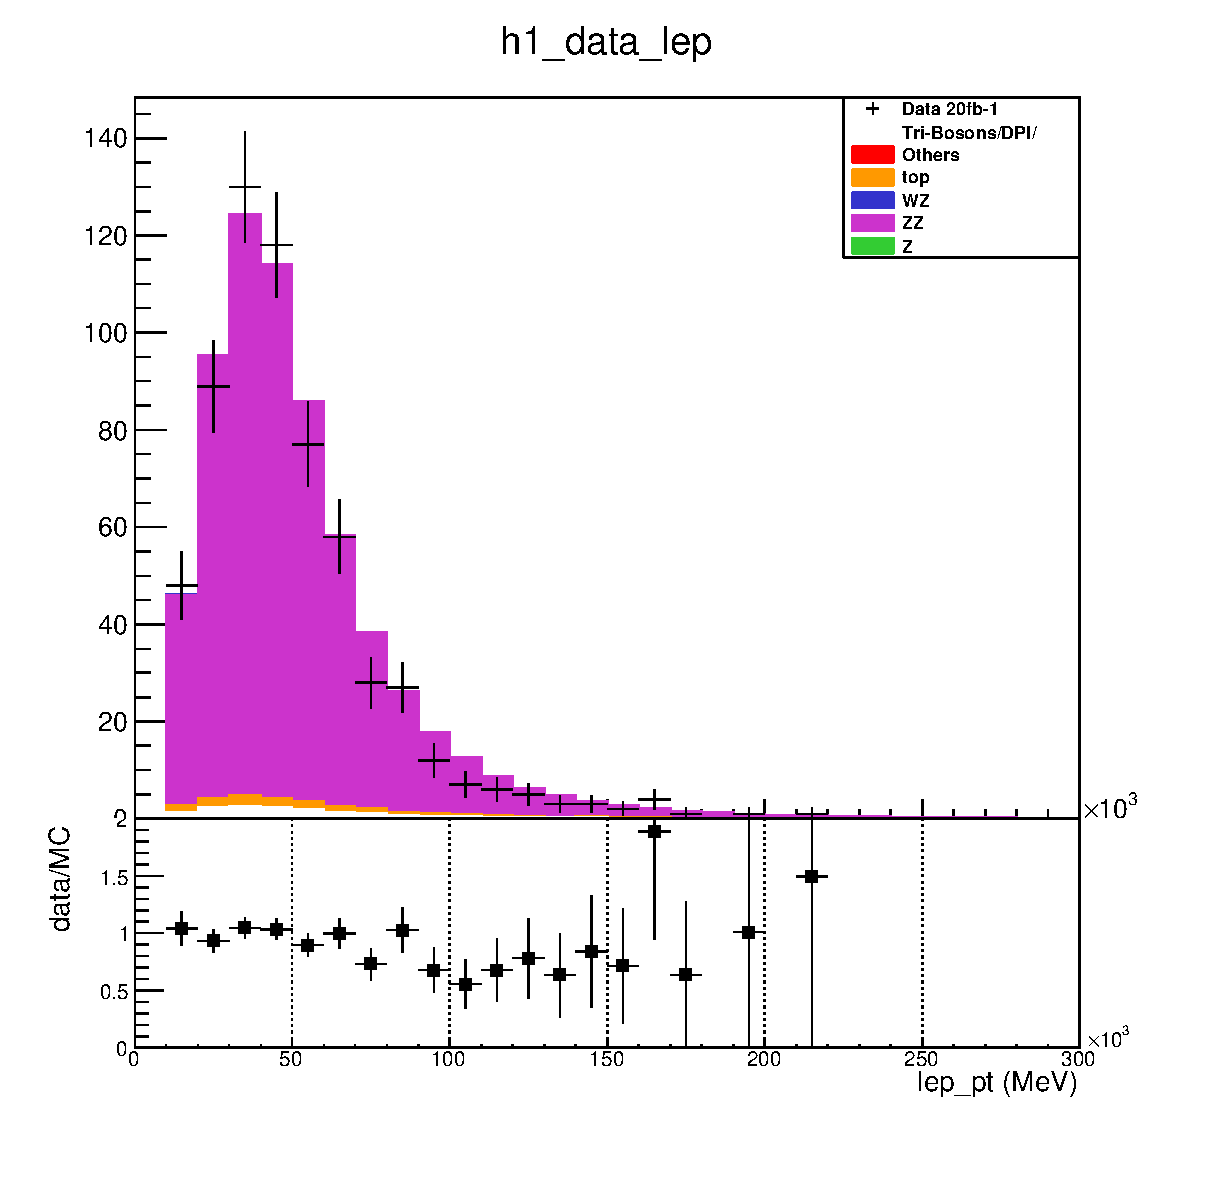
\includegraphics[width=0.4\textwidth]{figures/ZZ_CR/ZZ_CR_lep_pt.eps}
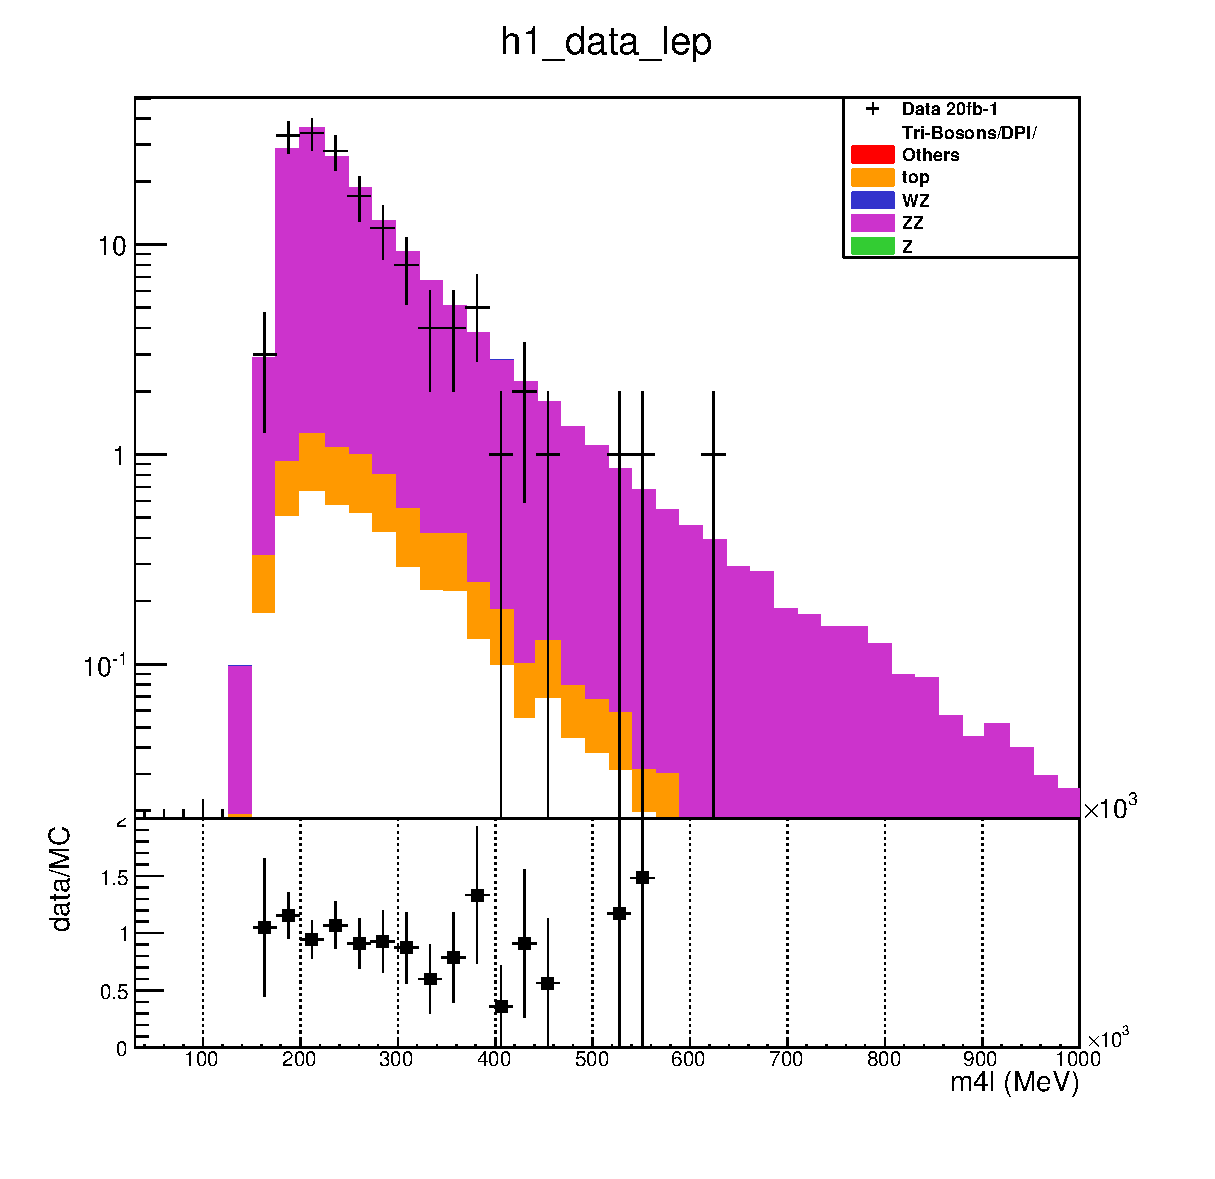
\includegraphics[width=0.4\textwidth]{figures/ZZ_CR/ZZ_CR_m4l.eps}
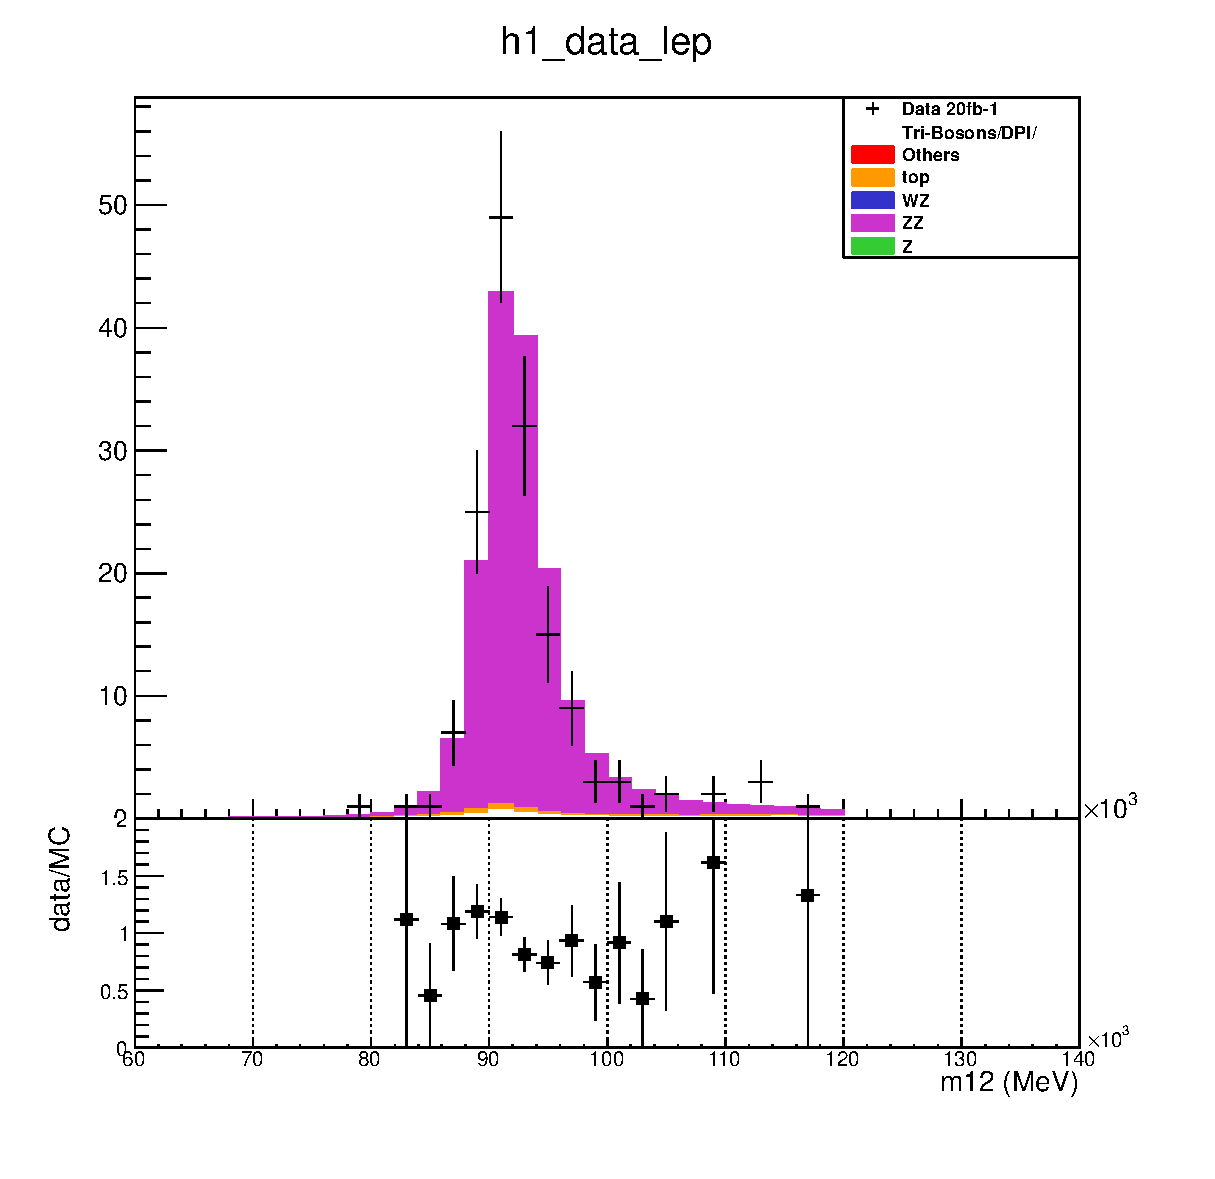
\includegraphics[width=0.4\textwidth]{figures/ZZ_CR/ZZ_CR_m12.eps}
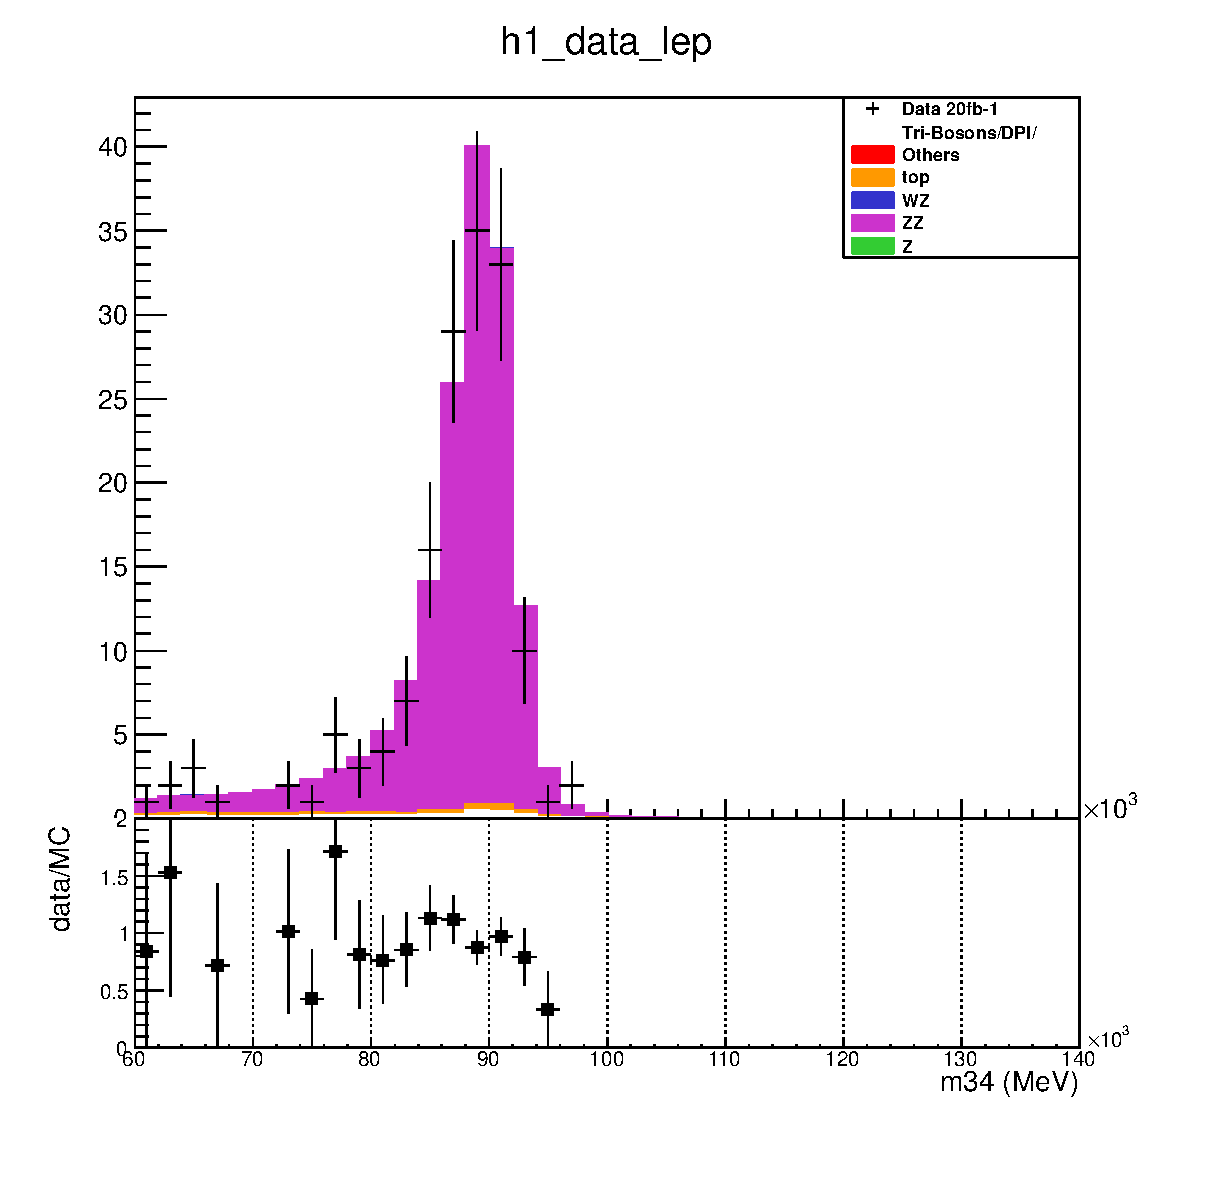
\includegraphics[width=0.4\textwidth]{figures/ZZ_CR/ZZ_CR_m34.eps}

\caption{$ZZ\to{}4\ell$ Control regions. Distribution of leptons $p_{T}$, $m_{12}$, $m_{34}$, $m_{4l}$.}
\label{fig:ZZ_CR}
\end{figure}  

\begin{table}[htp]
\centering
\begin{tabular}{|c||c|c|c|c|}
\hline
 & Event Yield\\ 
\hline\hline
$WZ$ &  $0.05 \pm 0.01$\\ 
$ZZ$ &  $156.2 \pm 0.3$(stat) $\pm 22.3$(syst) \\ 
% $gg2ZZ$ &	$21.3 \pm 0.2$ \\
$Z\gamma$ &  $0.0 \pm 0.0$\\ 
Fake (MC) &  $3.6 \pm 0.2$\\ 
triboson and $t\bar{t}+V$ &  $4.1 \pm 0.2$\\ 
\hline
Expected Signal + Background &  $164.0 \pm 0.3$ (stat) $\pm 22.3$(syst)\\ 
\hline
Observed Data &  $155 \pm 12$\\ 
\hline
\end{tabular}
\caption{Number of data and predicted events in the ZZ CR. The error quoted on the MC samples represents only the statistical error on the MC samples. The systematic error due to theoretical normalization on the $ZZ$ sample is also showed.}
\label{tab:ZZ_CR}
\end{table}


\clearpage

\subsubsection{$Z\gamma$}

The $Z\gamma$ process, where the $Z$ boson decays to a pair of leptons ($e$ and $\mu$), is estimated from MC. This proces is obtained using the Sherpa generator. It was found that Sherpa describes accurately the shape and normalization of data in the $7~\TeV$ and $8~\TeV$ datasets~\cite{Aad:2013izg,Auerbach:1631102}. Therefore the normalization of these sample is taken to be the cross-section provided by the Sherpa generator. These processes are contributing to our selection, via the conversion of one photon into a pair of electrons, and then the loss of one of these electrons in the acceptance. 

These effects are expected to be properly described by the simulation, but the agreement between the data and the model is checked in a control region where the events are requested to contains exactly two muons and one electron, and the tri-body invariant mass of this system, should be close to the $Z$-pole mass~\cite{PDG:2014}: $|m_{\mu\mu{}e}-91.19|<15~\GeV$.

Figure~\ref{fig:Zgamma_CR} shows the invariant mass distribution of the 3 leptons, the leptons $p_{T}$, the $\eta$ distribution of the electron, and the jet multiplicity. The normalization in the CR is also checked and is provided in Table~\ref{tab:Zgamma_CR}.
All the distributions and the event yield show a very good agreement between the data and the model.

\begin{figure}[htp]
\centering
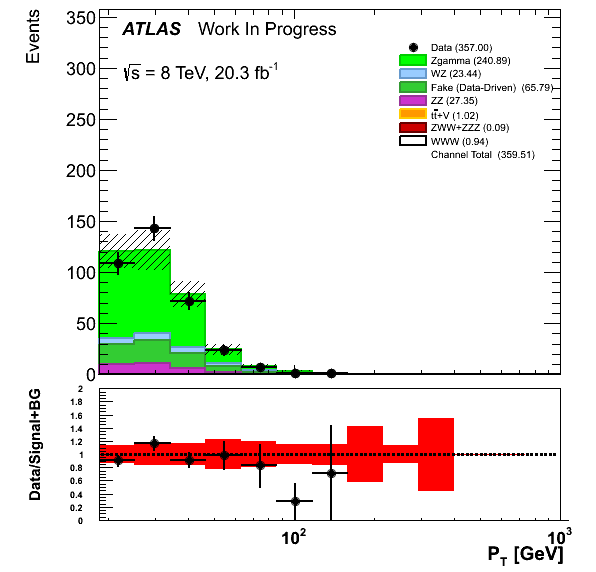
\includegraphics[width=0.4\textwidth]{figures/ZG_CR/AllLeptonPt_histratio.png}
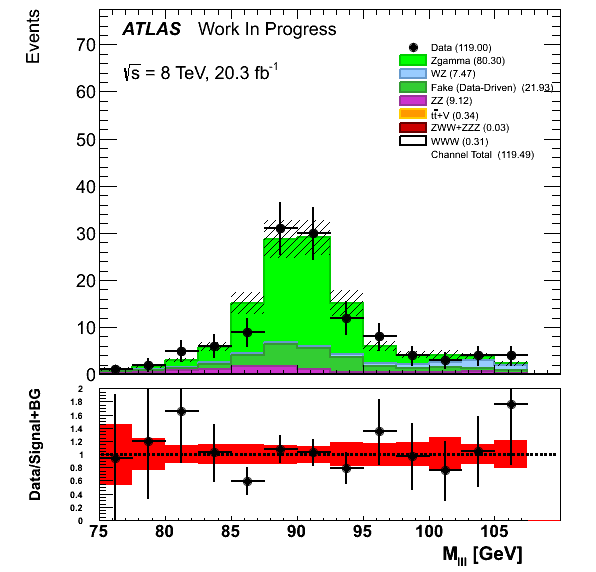
\includegraphics[width=0.4\textwidth]{figures/ZG_CR/InvariantMassThreeLep_histratio.png}
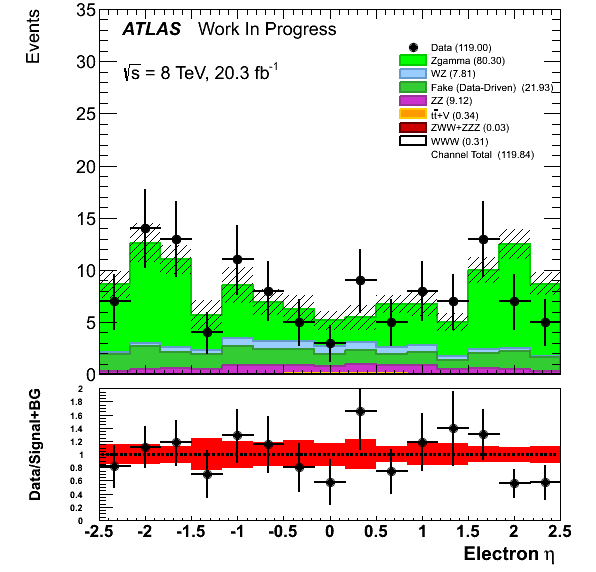
\includegraphics[width=0.4\textwidth]{figures/ZG_CR/ElectronEta_histratio.png}
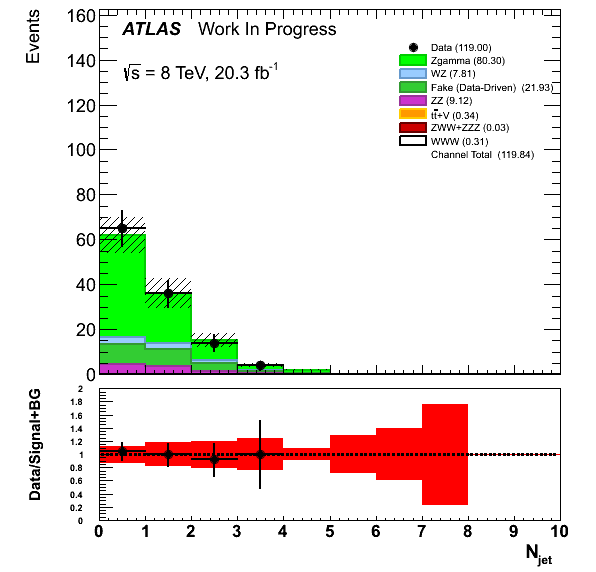
\includegraphics[width=0.4\textwidth]{figures/ZG_CR/NJets_histratio.png}

\caption{$Z\gamma$ Control region. Distribution of leptons $p_{T}$, invariant mass of the 3leptons, electron $\eta$, and jet multiplicity.}
\label{fig:Zgamma_CR}
\end{figure}  


\begin{table}[ht!]
\centering
\begin{tabular}{|c||c|c|c|c|}
\hline
 & Event Yield\\ 
\hline\hline
$WZ$ &  $7.47 \pm 0.11$\\ 
$ZZ$ &  $9.116 \pm 0.075$\\ 
$Z\gamma$ &  $80.3 \pm 2.8$\\ 
$ZWW+ZZZ$ &  $0.0285 \pm 0.0046$\\ 
$t\bar{t}+V$ &  $0.338 \pm 0.012$\\ 
Fake (data-driven) &  $21.9 \pm 1.2$\\ 
$WWW$ &  $0.3142 \pm 0.0072$\\ 
\hline
Expected Background &  $119.2 \pm 3.1$\\ 
Expected Signal + Background &  $119.5 \pm 3.1$\\ 
\hline
Observed Data &  $119 \pm 11$\\ 
\hline
\end{tabular}

\caption{Expected and observed event yields for the Z$\gamma$ control region. Only the statistical uncertainties are showed.}
\label{tab:Zgamma_CR}
\end{table}



\subsubsection{Double parton scattering, $\ttbar + V$, and $VVV$}

\paragraph{DPS}
\label{sec:bkg_DPS}
Double parton scattering (DPS) backgrounds are also taken into account in the analysis. To estimate their contribution a list of samples used in the same sign WW analysis~\cite{Aad:2014zda,DPS:Twiki} has been used. The cross section of these processes can not be taken directly from MC, but it must be further studied. Considering the DPS production of $A+B$, where $A$ and $B$ can be products of any single-parton, the cross section can can be factorised as~\cite{Gaunt:2010pi}:
\begin{equation}
	\sigma^{DPS}_{(A+B)}=\frac{m}{2}\times{}\frac{\sigma^{S}_{A}\times{}\sigma^{S}_{B}}{\sigma_{eff}}
\end{equation}	

Where $\sigma^{S}_{(A/B)}$ is the single-parton scattering production cross-section of the procss $A/B$, $m$ is a factor which takes the value of 1 when $A=B$ and 2 when $A\ne B$, $\sigma_{eff}$ is the effective cross section of the proton. A measurement of $\sigma_{eff} =15\pm3(stat)^{+5}_{-3}(syst)$ mb for 7~\TeV{} $p-p$ collisions has been recently performed by ATLAS~\cite{Aad:2013bjm}. By factorising the cross-section in this form, the correlation between the two parton interactions are neglected.

The samples and cross section that have been used in this analysis are given in Table~\ref{tab:sample_bkg_dibosons_gg2DPI}. An uncertainty of $50\%$ is applied on the normalization of these processes. Among these processes the one that can give a trilepton final state are: $WZ$, $ZZ$, and $Z\gamma$.
	
Their contributions are found to be negligible.


\paragraph{Other backgrounds}
The other backgrounds evaluated from MC are the one containing three real leptons: $t\bar{t}+V$, $WWZ$, and $WZZ$.
The PDF and scale uncertainties for the $t\bar{t}+V$ processes have been evaluated by other member of the ATLAS collaboration~\cite{ttV:Twiki}, and found
to be about $30\%$ of their normalization. These processes have been recently measured by the ATLAS collaboration~\cite{ATLAS-CONF-2015-032}, and their normalization are found to be consistent with the NLO predictions.

An equivalent $30\%$ uncertainty is assigned for the other $VVV$ contributions ($ZWW^{*}$ and $ZZZ^{*}$) that are not coming from our signal.

% Other background contributions are arising from tt¯+V, t+V and VVV processes. They will be estimated
%  using MC samples and global normalisation uncertainties are associated to these MC predictions. An
%  uncertainty of 30\% is assigned to the tt¯+ V contribution, according to [27]. An uncertainty of 30\% is
%  also assigned to the VVV contribution.
